\setAuthor{Aigar Vaigu}
\setRound{piirkonnavoor}
\setYear{2008}
\setNumber{G 6}
\setDifficulty{8}
\setTopic{Dünaamika}

\prob{Klaaskuul}
Klaaskuul kukkus vertikaalselt alla libedale horisontaalsele põrandale ning purunes kolmeks tükiks, mis lendasid mööda põrandat laiali. Sündmus jäädvustati fotol (vt joonist). Tükkide kujutised osutusid välja venitatuks, sest säriaeg oli võrdlemisi pikk. Millised olid kuuli tükkide masside suhted? Hõõrdejõud tükkide liikumisel lugeda tühiselt väikeseks. Fotoobjektiivi optiline peatelg oli pildistamisel vertikaalne

\begin{center}
	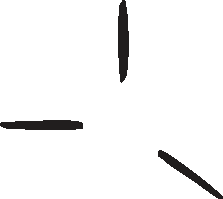
\includegraphics[width=0.6\linewidth]{2008-v2g-06-yl}
\end{center}

\hint
Tükikeste trajektooride järgi saab võrrelda kiiruste suundasid ja suuruseid, sest $s = vt_s$, kus $t_s$ on säriaeg. Lisaks kehtib impulsi jäävus. Kuna klaaskuul kukkus otse alla, peab summaarne põrandaga paralleelne impulss olema 0.

\solu
Tükikeste trajektooride järgi saab võrrelda kiiruste suundasid ja suuruseid, sest $s = vt_s$, kus $t_s$ on säriaeg (alternatiivselt võib kasutada kaugust kukkumispunktist $S = vt_S$, kus $t_S$ on ajavahemik mahakukkumishetkest säriaja lõpuni). Seega on jälgede pikkuste suhe (või jälgede lõpp-punktide kauguste suhe kukkumispunktist) võrdne kiiruste suhtega. Fotolt saame, et $s_1 \approx s_2 \approx s_3$, st $v_1 \approx v_2 \approx v_3$. Kuna kiiruste suunad on teada, siis on teada ka impulsside $\vec p_1 = m_1\vec v_1$, $\vec p_2 = m_2\vec v_2$ ja $\vec p_3 = m_3\vec v_3$ suunad. Kuna $\vec p_1 + \vec p_2 + \vec p_3 = 0$, siis moodustavad need vektorid kolmnurga. Et selle kolmnurga külgede suunad on teada, siis on teada selle kolmnurga nurkade suurused ning kolmnurk määratud sarnasusteguri täpsusega (et meid huvitavad külgede pikkuste suhted, siis sellest täpsusest piisab). Niisiis konstrueerime fotole kolmurga, mille küljed on vastavalt paralleelsed kolme kuulikillu jäljega. Jooniselt leiame, et $p_1 : p_2 : p_3$ suhtuvad kui $3 : 4 : 5$. Kombineerides seda nüüd eelmise tulemusega $v_1 \approx v_2 \approx v_3$ saame, et $m_1 : m_2 : m_3$ suhtuvad kui $3 : 4 : 5$.
\begin{center}
	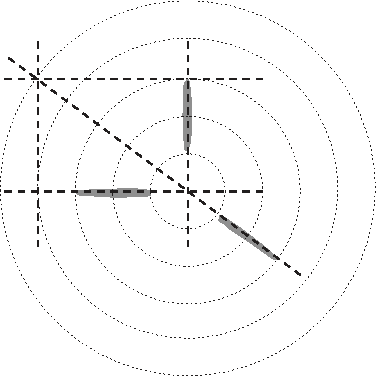
\includegraphics[width=0.6\linewidth]{2008-v2g-06-lah}
\end{center}
\probend